\documentclass[12pt]{article}
\usepackage[utf8]{inputenc}
\usepackage[T1]{fontenc}

\usepackage{bm}							% bold math symbols
\usepackage{amsmath}					% equation formatting
\usepackage{amssymb}					% equation symbols
\usepackage{mathtools}					% amsmath extension, symbols
\usepackage{siunitx}					% SI units package
\usepackage{caption}					% extended caption functionality
\usepackage{subcaption}					% provides subcaptions
\usepackage{graphicx}					% images
\usepackage{xcolor}						% driver-independent colors
\usepackage{wrapfig}					% figure wrapping
\usepackage{tikz}						% portable graphics format creator
\usetikzlibrary{decorations.pathreplacing}

\usepackage[margin=1in]{geometry}		% document layout package

\usepackage[notes,backend=biber]{biblatex-chicago} % citation styling
\usepackage[english]{babel}				% language package
\usepackage[autostyle=true]{csquotes}	% extended quotation functionality
\usepackage{hyperref}					% hypertext support

\usepackage{setspace}					% easy text spacing
%\usepackage{newtxtext,newtxmath} 		% times new roman, more up to date

% Standard ihat and jhat are not implemented by default.
% This provides the ihat and jhat without the dot at the top.
% Is basic implementation, does not work with mathptmx
%\newcommand{\ihat}{\mathbf {\hat \imath}}
%\newcommand{\jhat}{\mathbf {\hat \jmath}}

% Declare bibliography as the 'references.bib' file
\bibliography{references}

% Set doublespacing
\doublespacing
%\renewcommand{\baselinestretch}{1.5}

% Custom text formatting
\setlength{\parindent}{0pt}
\setlength{\parskip}{1em}

% Renaming the 'Contents' field to 'Table of Contents'
\addto\captionsenglish{ % required by babel
	\renewcommand{\contentsname}{Table of Contents}
}

% implementation of a unit vector as given by 'egreg' from tex.stackexchange.com 
% https://tex.stackexchange.com/questions/188775/how-to-type-a-particular-kind-of-unit-vector
\newcommand{\uveci}{{\bm{\hat{\textnormal{\bfseries\i}}}}}
\newcommand{\uvecj}{{\bm{\hat{\textnormal{\bfseries\j}}}}}
\DeclareRobustCommand{\uvec}[1]{{%
		\ifcat\relax\noexpand#1%
		% it should be a Greek letter
		\bm{\hat{#1}}%
		\else
		\ifcsname uvec#1\endcsname
		\csname uvec#1\endcsname
		\else
		\bm{\hat{\mathbf{#1}}}% This really is the only important thing
		\fi
		\fi
}}

% PREFERED COMPILER: XeLaTeX!

\newcommand{\bvec}[1]{\bm{\mathbf{#1}}}

\captionsetup[figure]{font=small,justification=centering}

\allowdisplaybreaks

\begin{document}
	\begin{titlepage}
	\begin{center}
		\vspace*{\fill}
		
		The Mathematical Exploration of Lagrange Points
		
		\vspace*{1.0cm}
		Word Count: 2656
		
		\vfill
		
		%Julian Joaquin\\
		Candidate Number: JYZ314\\
		Mathematics SL \\
		%Westwood Collegiate \\
		May 2022
		
		\vspace*{\fill}
		
	\end{center}
\end{titlepage}

	
	\tableofcontents
	
	\newpage
	
	\section{Introduction}
	
	In this day and age, the aerospace industry has become a vital component of the global economy.
In a publication by the Organisation for Economic Co-operation and Development, the space economy plays a key role in the globalization and digitization of the modern world, with space activities making crucial contributions to the social, economic, and scientific aspects of society\autocite{c5996201-en}.
With an increasing investment for spaceflight, there is future need to develop infrastructure that can facilitate the growing space sector, which includes the necessity to understand the nature of orbital mechanics.

Since the longest time, I've always been interested in the development of spaceflight.
There's a sort of cosmic beauty with how objects behave in space, subject predominantly and almost exclusively to the fundamental force that is gravity.
And it is also because of this exclusivity to a single force that makes it ripe for mathematical exploration.
In particular, the launch of the James Webb Space Telescope is a unique mission where the space telescope will sit \textit{behind} the Earth relative to the Sun, in orbit around the Lagrange point L2.
This stands against high school intuition that objects in space orbit around bodies with mass; somehow, the JWST is able to exist in a (somewhat) stable orbit around seemingly nothing!
It is for this reason that this investigation aims to explore the mathematics behind Lagrange points.
More specifically, I seek to learn about the nature of Lagrange points, specifically L2, from a basic physics understanding; an understanding through my mathematical knowledge from school; and from a higher level of mathematics such that we can model what the orbit around a collinear Lagrange point would look like.

It is important to note that this paper does not seek out to give a method which can accurately predict the motion of an object in space with clear solutions; there exists a good reason why orbital mechanics is not taught in detail in high school.
Instead, this paper investigates Lagrange points in such a way that allows for a conceptual understanding that can still facilitate for numerical computations of the motion of objects near a collinear Lagrange point.
It is also due to the complexity of this investigation that more advanced utilities will be used.
Primarily, Python libraries will be used for numerical computations of large numbers, numerical approximation of equations with no solutions, and graphing three-dimensional space.
	
	\section{Finding the Lagrange Points}
	
	From a basic understanding of classical mechanics, we can determine the location of Lagrange points. Before we do any math on Lagrange points, its important to know what they are exactly. According to NASA, Lagrange points are special solutions in what is know as the ``three-body problem.'' At these points in space, the gravitational and rotational forces of the other two bodies effectively cancel each other out, allowing small objects to seemingly stay in place\autocite{JWSTOrbit}.

With this in mind, lets consider a simple system of two static masses, $m_1$ and $m_2$, where $m_1 > m_2$.

\vspace*{0.5cm}
\begin{figure}[!h]
	\centering
	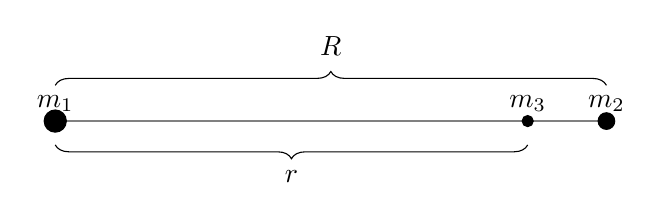
\begin{tikzpicture}
		\draw[gray,thick] (-4,0) -- (3,0);
		\filldraw (-4,0) circle (4pt) node[anchor=south]{$m_1$};
		\filldraw (3,0) circle (3pt) node[anchor=south]{$m_2$};
		\filldraw (2,0) circle (2pt) node[anchor=south]{$m_3$};
		\draw[decorate,decoration={brace,amplitude=5pt,raise=3ex}] (-4,0) -- (3,0) node[midway,yshift=27pt]{$R$};
		\draw[decorate,decoration={brace,mirror,amplitude=5pt,raise=2ex}] (-4,0) -- (2,0) node[midway,yshift=-2em]{$r$};
	\end{tikzpicture}
	\vspace*{0.25cm}
	\caption{System of two stationary bodies.}
	\label{fig:collinear-coords}
\end{figure}

In Figure \ref{fig:collinear-coords}, $R$ represents the distance between the two bodies, and $r$ represents the distance from the first body to the equilibrium point, point mass $m_3$, where the net gravitational force is 0. Using Newton's Law of Gravitation,
\begin{equation*}
	F = \frac{Gm_1m_2}{r^2}
\end{equation*}
where F is the force exerted between two bodies of mass and G is the gravitational constant, we can write the net force of the system as:
\begin{equation*}
	\frac{Gm_1m_3}{r^2} = \frac{Gm_2m_3}{(R - r)^2}
\end{equation*}
If we let $m_1 = 4m_2$ and $R = 1$, than we can directly solve for $r$:
\begin{align*}
	\frac{m_1}{r^2} &= \frac{m_2}{(R - r)^2} \\
	\left(\frac{R - r}{r}\right)^2 &= \frac{m_2}{m_1} \\
	\left(\frac{1 - r}{r}\right)^2 &= \frac{m_2}{4m_2} \\
	\frac{1 - r}{r} &= \frac{1}{2} \\
	2 - 2r &= r \\
	\frac{2}{3} &= r
\end{align*}
Of course, this scenario is not exemplary of Lagrange points, let alone the interaction between celestial bodies. Let us increase the complexity of our initial system by placing $m_2$ in a circular orbit around $m_1$. With consideration for rotational force, centripetal force is expressed as:
\begin{equation*}
	F = \frac{4\pi^2m_3r}{T^2}
\end{equation*}
where $T$ expresses the orbital period of $m_3$. Given that, from Kepler's Third Law,
\begin{equation*}
	T = 2\pi \sqrt{\frac{R^3}{G(m_1 + m_2)}}
\end{equation*}
centripetal force can be rewritten as:
\begin{equation*}
	F = \frac{G(m_1+m_2)}{R^3}rm_3
\end{equation*}
Therefore, the net force between $m_1$ and $m_2$ is written as:
\begin{equation*}
	F = m_3a = -\frac{Gm_1m_3}{r^2} - \frac{Gm_2m_3}{(r - R)^2} + \frac{G(m_1+m_2)}{R^3}rm_3
\end{equation*}
Solving for the centripetal acceleration, we get the formula:
\begin{equation*}
	a = -\frac{Gm_1}{r^2} - \frac{Gm_2}{(r - R)^2} + \frac{G(m_1+m_2)}{R^3}r
\end{equation*}
Most of the variables are known constants, with \textit{r} being the only unknown value which represents the distance of the Lagrange point from $m_1$, given that the net radial acceleration is 0.
It is worth noting that, with respect to direction, $r^2$ and $(r-R)^2$ will only reflect acceleration due to gravity in the negative direction and will not be sufficient to tell us where L1 and L3 are.
Knowing that, cautiously, $n^2 = n \times |n|$, the formula is rewritten as such to preserve the sign of $r$:
\begin{equation}
	a = -\frac{Gm_1}{r|r|} - \frac{Gm_2}{(r - R)|r - R|} + \frac{G(m_1+m_2)}{R^3}r \label{eqn:x-accel1}
\end{equation}
To save ourselves the agony of whether it is possible to isolate for $r$, we will use Python to plot the centripetal acceleration with respect to distance. The Lagrange points are located where the acceleration is 0.
\begin{figure}[H]
	\centering
	\captionsetup[subfigure]{justification=centering}
	\begin{subfigure}[b]{0.4\textwidth}
		\centering
		\includegraphics[scale=0.6]{r-accel-figure-1.png}
		\caption{\footnotesize Radial acceleration between the Sun and Earth.}
		\label{fig:radial-accel-system}
	\end{subfigure}
	\hspace*{1cm}
	\begin{subfigure}[b]{0.4\textwidth}
		\centering
		\includegraphics[scale=0.6]{r-accel-figure-2.png}
		\caption{\footnotesize Radial acceleration around the Earth.\vspace*{1.16em}}
		\label{fig:radial-accel-earth}
	\end{subfigure}
	\label{fig:radial-accel}
	\caption{Net radial acceleration vs distance of the Sun-Earth system. Graphs are created using the matplotlib Python library.}
\end{figure}
Given that we are only concerned with L2, the distance of L2 from the Sun is computed as $1.511 \times 10^8 \si{\kilo\metre}$.

Note how Equation \eqref{eqn:x-accel1} for acceleration is dependent on the distance an object is from either body.
Should we try to predict the motion of an object, there would be no way to express distance as a function of time.
This is a major hurdle that occurs in physics and, while there can be specific situations where this can be overcome, most of the time there is no solution.
Instead, we would have to numerically integrate the distance travelled over time.
Not to be confused with integration, this means that we would need to calculate the acceleration at a certain distance, let our object travel for an interval of time at said acceleration, than recalculate acceleration for our new distance.
This is tedious work that, for the sake of both my sanity and time, we will delegate to computers.
We should not let this caveat daunt us, however, as there is still a lot to learn about how we describe the motion of objects in such a relation.

%\begin{figure}[!h]
%	\centering
%	\begin{tikzpicture}
%		\draw[grey,thick] (0,0) circle (2);
%		\filldraw (0,0) circle (3pt) node[anchor=north east]{$m_1$};
%		\filldraw (1.41, 1.41) circle (2pt) node[anchor=south west]{$m_2$};
%		\draw[thick,<-] (0.71,0.71) -- (1.41,1.41);
%		\node at (0.71, 0.71) [below,align=right]{$a$};
%	\end{tikzpicture}
%\vspace*{0.25cm}
%\caption{Orbit of }
%\label{fig:orbit}
%\end{figure}
	
	\section{Setup Scenarios for Equations of Motion}
	
	As stated in the introduction, finding out the motion of a satellite around a Lagrange point will be incredibly difficult.
To prepare for this, let us take a step back and tackle these two scenarios.

\subsection{Simple Linear Differential Equations} \label{sec:ode}

For our first scenario, let us imagine that, for some function $n$ with respect to $t$,
\begin{equation}\label{eqn:lde1}
	\frac{dn}{dt} = 4n
\end{equation}
In words, the rate of change of the function is equal to itself multiplied by four. Let us say we wanted to find what function $n$ is.
While it is not as simple to just integrate this equation, we know that $e^x$ is its own derivative.
We also know that, because of the chain rule, $[e^{kt}]' = ke^{kt}$.
If we substitute $n$ for $e^{kx}$ and let $k = 4$, then equation \eqref{eqn:lde1} is true.
Therefore, we can state the following theorem; for some equation
\begin{equation}\label{eqn:theory1}
	\frac{dn}{dt} = kn\ \text{,} \quad n = ce^{kt}
\end{equation}
where $c$ is some initial constant that cannot be expressed from integrating the derivative.
We can verify that this theorem is correct using some algebra and integration.
\begin{align*}
	\frac{dn}{dt} &= kn \\
	\frac{1}{n}\, dn &= k\, dt \\
	\int \frac{1}{n}\, dn &= \int k\, dt \\
	\ln n + C &= kt + D \\
	\ln n &= kt + (D - C) \\
	n &= e^{kt} \cdot e^{D - C} \hspace*{3em}
\end{align*}
This will become handy for equations that are only defined by their derivative.

\subsection{Systems of Linear Differential Equations} \label{sec:ode-sys}

The second scenario builds off the first, and involves equations that are defined by each other.
Consider the following system of equations with functions $x$ and $y$ in terms of $t$:
\begin{align*}
	\frac{dx}{dt} &= 4x - 2y \quad &x(0) = 4 \\
	\frac{dy}{dt} &= 3x - y \quad &y(0) = 2
\end{align*}
Here, the rate of change of $x$ is defined in terms of both $x$ and $y$, and same goes for the rate of change of $y$.
Because these two equations are intertwined, initially it seems impossible to define both $x$ and $y$ as separate from each other.
However, remembering our previous theorem, Equation \eqref{eqn:theory1}, we can predict that both functions will look something like this:
\begin{align}
	x(t) = c_1e^{r_1t} + c_2e^{r_1t} \label{eqn:x-t-general}\\
	y(t) = c_1e^{r_2t} + c_2e^{r_2t} \label{eqn:y-t-general}
\end{align}
Also from Equation \eqref{eqn:theory1}, let us imagine that it is possible to state the rate of change as function of itself multiplied by a constant, $k$.
\begin{align}
	\frac{dx}{dt} &= kx = 4x - 2y \label{eqn:kx-sys}\\
	\frac{dy}{dt} &= ky = 3x - y \label{eqn:ky-sys}
\end{align}
Forgetting the fact that we are involving derivatives for a moment, we can try solving for $k$ by solving this linear system though substitution.
\begin{align}
	4x - 2y &= kx \nonumber \\
	(4 - k)x &= 2y \nonumber \\
	\frac{(4 - k)x}{2} &= y \nonumber \\
	3x - y &=ky \nonumber \\
	3x &= (k + 1)y \nonumber \\
	3x &= (k + 1)\frac{(4 - k)x}{2} \nonumber \\
	3\cdot2 &= (k + 1)(4 - k) \nonumber \\
	0 &= (1 + k)(4 - k) - 3\cdot2 \label{eqn:chr-polynomial-ex}
\end{align}
By now, we can deduce that there will be two possible values for $k$.
Continuing the solution,
\begin{align*}
	0 &= -k^2 - 3k + 2 \\
	0 &= (k - 1)(k - 2)
\end{align*}
Here, the solutions are $k_1 = 1$ and $k_2 = 2$.
We don't know exactly what these values \textit{mean}, other than they correspond to $x$ and $y$, respectively.
Let us see what happens when we plug them into our linear system.
For $k_1$:
\begin{equation*}
	\left. \begin{array}{l}
		(1)x = 4x - 2y \\
		(1)y = 3x - y
	\end{array} \right \}
	\implies 0 = 3x - 2y \implies 2y = 3x
\end{equation*}
This gives us a relationship of $x$ and $y$ where, when $k = 1$, there is a 
$2 : 3$ ratio between $x$ and $y$.
This is significant because, for some specific values of $x$, $y$, and $k$, our system of linear equations \textit{converge} in a manner that essentially defines them as the same equation.
This is easier to understand when graphed.
\begin{figure}[h!]
	\centering
	\captionsetup[subfigure]{justification=centering}
	\begin{subfigure}[b]{0.4\textwidth}
		\centering
		\begin{tikzpicture}
			\draw (-3,0) -- (3,0) node[right] {$x$};
			\draw (0,-3) -- (0,3) node[above] {$y$};
			\draw[thick,green] (-1.5, -3) -- (1.5,3);
			\draw[thick,dashed,red] (-1,-3) -- (1,3);
			\node at (1,-1) [right,align=right] {$\textcolor{green}{4x - 2x = kx}$ \\
				$\textcolor{red}{3x - y = ky}$ \\
				$\textcolor{black}{k = 0}$};
		\end{tikzpicture}
		\caption{\small Linear system with $k = 0$.}
		\label{fig:sample-eigens0}
	\end{subfigure}
	\qquad
	\begin{subfigure}[b]{0.4\textwidth}
		\centering
		\begin{tikzpicture}
			\draw (-3,0) -- (3,0) node[right] {$x$};
			\draw (0,-3) -- (0,3) node[above] {$y$};
			\draw[thick,green] (-2, -3) -- (2,3);
			\draw[thick,dashed,red] (-2,-3) -- (2,3);
			\filldraw[black] (1,1.5) circle (1.25pt) node[anchor=west] {$\textcolor{black}{(2,3)}$};
			\node at (1,-1) [right,align=right] {$\textcolor{green}{4x - 2x = kx}$ \\
				$\textcolor{red}{3x - y = ky}$ \\
				$\textcolor{black}{k = 1}$};
		\end{tikzpicture}
		\caption{\small Linear system with $k = 1$.}
		\label{fig:sample-eigens1}
	\end{subfigure}
	\caption{The linear system defined with regard to $k$. (It is better to think of the graphs as ratios between $x$ and $y$ rather than $y$ as a function of $x$.)}
	\label{fig:sample-eigens}
\end{figure}
In Figure \ref{fig:sample-eigens0}, you can see how, for other values of $k$, the ratios between $x$ and $y$ are different, whereas in Figure \ref{fig:sample-eigens1}, the ratios are the same at $2 : 3$ when $k$ specifically equals 1.
This means we can express the $x$ term of both functions $x$ and $y$ separately for specific values of $k$, which would be 1 and 2.
In terms of Equations \eqref{eqn:x-t-general} and \eqref{eqn:y-t-general}, the $x$ term of the function $x$ will have the additional coefficient of 2 while the $x$ term in the function $y$ will have the additional coefficient of 3.
Therefore, we can add the following to Equations \eqref{eqn:x-t-general} and \eqref{eqn:y-t-general}:
\begin{align}
	x(t) = (2)c_1e^{r_1t} + n_3c_2e^{r_2t} \label{eqn:x-t-partial} \\
	y(t) = (3)c_1e^{r_1t} + n_4c_2e^{r_2t} \label{eqn:y-t-partial}
\end{align}
where $n$ expresses the necessary coefficients for each ratio. What role does $k$ play in the solution? To figure out, first we will find the ratio for when $k = 2$.
\begin{equation*}
	\left. \begin{array}{l}
		(2)x = 4x - 2y \\
		(2)y = 3x - y
	\end{array} \right \}
	\implies 0 = x - y \implies y = x
\end{equation*}
Here, there is a $1 : 1$ ratio between $x$ and $y$. What happens when we enter initial values for $x$ and $y$ that adhere to this ratio? For example, when $x = 2$ and $y = 2$:
\begin{gather*}
	4(2) - 2(2) = 8 - 4 = 4 \\
	3(2) - (2) = 6 - 2 = 4 
\end{gather*} % Do we need to set the equations equal to x and y?
It is as if the initial values were multiplied by the $k$ value!
This is actually expected, given how we laid out Equations \eqref{eqn:kx-sys} and \eqref{eqn:ky-sys}.
In this case, $k$ is the common coefficient between both $x$ and $y$ for the derivative of the function $y$.
\begin{equation*}
	\frac{dy}{dt} = 2y % THIS NEEDS TO BE CORRECTED!!!!
\end{equation*}
This essentially means $k$ can be used as the $r$ values from Equations \eqref{eqn:x-t-general} and \eqref{eqn:y-t-general}.
Finding the functions $x$ and $y$ is almost complete:
\begin{align*}
	x(t) = (2)c_1e^{(1)t} + (1)c_2e^{(2)t} \\
	y(t) = (3)c_1e^{(1)t} + (1)c_2e^{(2)t}
\end{align*}
All that is left is to find the initial constants for each equation given the initial values at the beginning of this scenario.
\begin{align*}
	\left. \begin{array}{l}
		x(0) = 4 = 2c_1 + c_2 \\
		y(0) = 2 = 3c_1 + c_2
	\end{array} \right\}
	&\implies 2 = -c_1 \implies -2 = c_1 \\
	2 = 3(-2) + c_2 &\implies 8 = c_2 \\
	x(t) =& -4e^t + 8e^{2t} \\
	y(t) =& -6e^t + 8e^{2t} 
\end{align*}
And that is the solution!
The reason why we want to understand how to solve this system is because we will encounter a similar system when deriving the equations of motion.
For that reason, we will also need a general method to solving these systems.

\subsection{General Theorems}

The key concepts that have been explored so far are the solution to a simple differential equation and solving a system of linear differential equations using eigenvalues and eigenvectors.
The objective of providing these scenarios is to develop an understanding of the concepts that will be used.
And indeed, the equations of motion that govern the movement around a Lagrange point are differential equations and will require the concepts above to solve numerically.
However, generalizing the concepts that have been applied so far, so that they can be applied to the equations of motion, will involve more concepts that will over-complicate this paper.
Therefore, the general theorems that will be applied for the equations of motion must sometimes be asserted.

Before the general theorems are established, is important to understand is how these concepts were used.
The first concept to know about is a differential equation; when an unknown function is defined alongside its derivative.
An applicable example of one is the simple equation explored in subsection \ref{sec:ode}, where the solution is an exponential function and whose solution is generalized in Equation \eqref{eqn:theory1}.
The second concept is a system of differential equations, where not only are there functions defined with relation to their derivatives, but also with relation to each other.
Equations \eqref{eqn:kx-sys} and \eqref{eqn:ky-sys} are a prime example of this.
The approach to the solution of these kinds of systems involves the third important concept, which is eigenvalues and eigenvectors.
The values of $k$ that were found in section \ref{sec:ode-sys} are known as eigenvalues and the ratios that were found alongside them are called eigenvectors.
The eigenvalues express, as single coefficients, how the system of equations effectively changes given values for each function with respect to the eigenvectors; the ratios between each function.
We can infer from Equation \eqref{eqn:chr-polynomial-ex} that, for two linear equations,
\begin{align*}
	\lambda x_1 &= ax_1 + bx_2 \\
	\lambda x_2 &= cx_1 + dx_2
\end{align*}
The eigenvalues, $\lambda$, are calculated as:
\begin{equation}
	0 = (a - \lambda)(d - \lambda) - bc
\end{equation}
For a system of three variables and three differential equations:
\begin{align*}
	\lambda x_1 &= ax_1 + bx_2 + cx_3 \\
	\lambda x_2 &= dx_1 + ex_2 + fx_3 \\
	\lambda x_3 &= gx_1 + hx_2 + ix_3
\end{align*}
The eigenvalues are calculated as:
\begin{align*}
	0 &= (a - \lambda)[(e - \lambda)(i - \lambda) - fh] + b[d(i - \lambda) - fg] - c[dh - (e - \lambda)g] \\
	&= (a - \lambda)(e - \lambda)(i - \lambda) + bfg + cdh - cg(e - \lambda) - bd(i - \lambda) - fh(a - \lambda)
\end{align*}
Notice how the calculation is, in essence, the calculation for the eigenvalues of three two-equation systems multiplied by the coefficients of the first top-most equation, $a, b, \text{and}\, c$.
This behaviour can be extrapolated onto the solution for a system of four variables and four differential equations with coefficients $(a_1, a_2, \dots, a_n)$,
%The key concepts explored through these scenarios are the solutions to systems of linear differential equations, and eigenvalues and eigenvectors.
%The first concept, differential equations, will appear when solving for the equations of motion and it is imperative that we understand how to approach them.
%We already know how to approach a single linear differential equation as stated from Equation \eqref{eqn:theory1}. However, when there are multiple differential equations that are defined in terms of each other, we will need eigenvalues and eigenvectors.

%As for the second concept, eigenvalues are the values of $k$ that we found, while eigenvectors are those special ratios between $x$ and $y$ where our system of equations converged to a single line on our graph back in Figure \ref{fig:sample-eigens1}.
%They are frequently discussed in linear algebra, where eigenvectors are specific vectors that maintain their direction after a linear transformation, and eigenvalues are the factor which the linear transformation scales the eigenvectors.
%However, linear algebra is significantly beyond the concern of this investigation.
%Eigenvalues and eigenvectors will be important for solving multiple differential equations who are defined by each other.
%We can infer from Equation \eqref{eqn:chr-polynomial-ex} that, for two linear differential equations,
%\begin{align*}
%	\frac{dx_1}{dt} = ax_1 + bx_2 \\
%	\frac{dx_2}{dt} = cx_1 + dx_2
%\end{align*}
%The eigenvalues, $\lambda$, are calculated as:
%\begin{equation}
%	0 = (a - \lambda)(d - \lambda) - bc
%\end{equation}
%We will need to generalize this for any number of differential equations, given that there exists only one differential equation for each unknown function.
%At this point, we have explored the concepts necessary to understand the solutions to systems of differential equations, and further exploration will expand beyond the aims of this paper.
	
	\newpage
	
	\section{Deriving Equations of Motion}
	
	Equations \eqref{eqn:eomx}, \eqref{eqn:eomy}, and \eqref{eqn:eomz} are our equations of motion that govern the movement of a satellite around a Lagrange point.
Technically, we can use them to represent motion anywhere in our system, not just around the Lagrange points.

Notice how the equations of motion are similar to \eqref{eqn:x-accel1}, where the distance, velocity, and acceleration of each dimension can not be represented separately as functions of time.
Still, it is possible to make use of these equations through numerical approximation.
This means that, given some initial conditions (position and velocity), the output is calculated (acceleration) for a small interval of time.
Than, after letting the new output determine the rest of the system for the said time interval, the output is recalculated with the given change from the initial conditions.
Recursively, this is generally written as:

\begin{equation*}
	y_{n+1} = y_n + hf(t_n)
\end{equation*}

where $h$ indicates the length of the time interval and where some value $y_0$ is known.
This particular equation is known as ``Euler's method''\autocite{BrilEulers} and is used to approximate equations that are similar to our equations of motion.
The method used to approximate the equations of motion will not specifically be Euler's method, but its purpose is practically identical.

$G$, $R$, $m_1$, $m_2$, and $\theta'$ are known constants, with the latter defined as:

\begin{equation*}
	\theta' = \omega = \sqrt{\frac{G(m_1 + m_2)}{R^3}} \text{,}
\end{equation*}

meaning the unknown values to the equations of motion are $x, y, z, x', y'$, and $z'$.
By setting our initial $x$ coordinate $(1.511\times10^{11} - 10^3)\si{\metre}$, $1000\si{\metre}$ away from of L2, and the remaining conditions $y, z, x', y', z' = 0$, we can compute our first trajectory for our satellite, $m_3$.
As seen in Figure \ref{fig:3dplot1}, the satellite unremarkably falls back towards the Earth.
This makes sense since there is no initial velocity and the initial position places it in the influence of Earth's gravity.
With these initial values, we can input them into our equations of motion and than numerically approximate the trajectories of our satellite using Python.
\newpage
\begin{samepage}
\begin{figure}[ht!]
	\centering
	\includegraphics[scale=0.52]{3dplot1.png}
	\caption{Trajectory plot of an object near L2 fo the Sun-Earth system, x-coordinate is $(1.511\times10^{11} - 10^3)\si{\metre}$, all other conditions are 0.
		The red point, $P_0$, indicates the starting position of the object.
		The black point indicates the Lagrange point.
		Generated through the matplotlib and scipy Python libraries.
	}
	\label{fig:3dplot1}
\end{figure}
In order to create a trajectory that resembles an orbit, we need to apply velocity that is perpendicular to the acceleration to create circular motion.
Knowing that $v^2 = ar$, we can write the equation:
\begin{equation*}
	u_y = a\sqrt{x''r}
\end{equation*}
where $u_y$ is the initial velocity in the $y$ component and $a$ is the proportionality constant, assuming that the orbit being predicted is not circular.
After some trial and error, $a = 2.2$ makes for a good approximation.
\begin{figure}[H]
	\centering
	\includegraphics[scale=0.52]{3dplot2.png}
	\caption{Trajectory plot of an object $1000\si{\metre}$ in the proximity of L2 in the Sun-Earth system in a semi-stable halo orbit.}
	\label{fig:3dplot2}
\end{figure}
\end{samepage}
And would you look at that; in Figure \ref{fig:3dplot2}, it seems as if our satellite orbits nothing!
Of course, it is also seen that the satellite eventually falls out of its orbit, confirming the instability of collinear Lagrange points.

We can now use this model and compare it to the actual trajectory of objects orbiting Lagrange points.
Given that telemetry of the JWST is readily available through JPL Horizons System, we will use its orbit for comparison.
\begin{figure}[H]
	\centering
	\captionsetup[subfigure]{justification=centering}
	\begin{subfigure}[b]{0.4\textwidth}
		\centering
		\includegraphics[scale=0.5]{3dplot3.png}
		\caption{Modelled trajectory plot of the JWST $2.5\times10^8\si{\metre}$ L2. Not modelled with station-keeping.}
		\label{fig:3dplot3}
	\end{subfigure}
	\qquad
	\begin{subfigure}[b]{0.4\textwidth}
		\centering
		\includegraphics[scale=0.2]{xyjwstplot.png}
		\vspace*{1em}
		\caption{Trajectory of the JWST according to the JPL Horizons database.}
		\label{fig:3dplot4}
		\vspace*{1em}
	\end{subfigure}
	\caption{Trajectories of the JWST. Figure (a) has $P_0$ positioned at $(L_2 - 2.5\times10^8, 0, - 1.2\times10^8)$. Figure (b) is generated through SageMath and produced by PM 2Ring on Stack Exchange.}
\end{figure}
Figure \ref{fig:3dplot3} is the trajectory of the JWST given the expected orbital characteristics prior to launch\autocite{JWSTHaloOrbit}.
Figure \ref{fig:3dplot4} is the trajectory of the JWST according to the JPL Horizons database from December 26th, 2021 to January 22, 2024\autocite{SEHaloOrbit}.
In Figure \ref{fig:3dplot3}, it is apparent that station-keeping, the use of onboard engines to stay on a specific orbit, is necessary for larger orbits around Lagrange points.
It is possible that a much more precise initial velocity approximations will produce a trajectory that stays in orbit for longer.
Still, the model seems to tend towards a similar elliptical, halo-like orbit that is shown in Figure \ref{fig:3dplot4}.
The difference in trajectories in both figures can be attributed to the degree of sophistication between our model and the model used by JPL.
This can include consideration for an elliptical, eccentric orbit of the Earth, the effects of the Moon's gravity, and orbital eccentricity of the JWST during its transfer to L2.
	
	\section{Plotting the Orbit}
	
	\section{Conclusion}
	
	\newpage
	
	\printbibliography[
	heading=bibintoc,
	title={References}
	]
	
\end{document}
